\section{Application of the Segmentation by Level Sets for Food Analysis}

We applied both snakes and level sets to segment the ketchup area of the dish.

We employed snakes with positive balloon force (i.e. inflating the curve from inside of the ketchup area). The first major drawback of snakes became obvious in the very first execution of the algorithm with the recommended parameters: the contour cannot perform topological changes. Therefore it cannot surround the small ingredients (``islands'', so to speak) in the middle of the dish without twisting over itself.
This is evidenced in figure \ref{fig:snakes-bad}. The best we could do to avoid this is to reduce the $ \lambda $ value from 0.05 to 0.04. The result is in figure \ref{fig:snakes-good}. Now the contour does not twist over itself, but the ketchup area is not completely segmented (still pretty good result taking into account that the contour cannot divide).

\begin{figure}[!hbt]
\centering   
\subfigure[Recommended parameters (with lambda positive)]{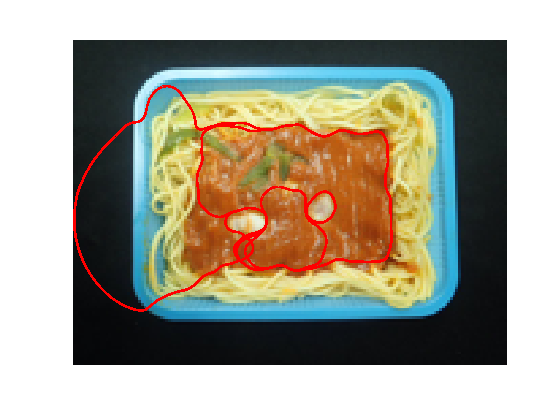
\includegraphics[width=60mm]{img/ex4/snakes_bad.png}\label{fig:snakes-bad}}
\subfigure[$ \lambda = 0.04 $]{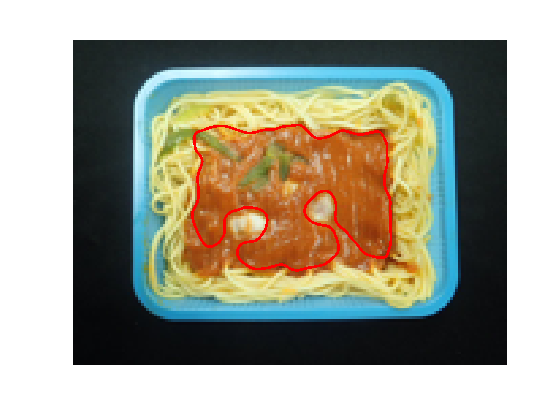
\includegraphics[width=60mm]{img/ex4/snakes_good.png}\label{fig:snakes-good}}
\caption{Segmentation of the dish with snakes}
\label{fig:snakes-dish}
\end{figure}

Without any doubt the best segmentations are obtained with level sets. In order to make it work correctly we need to set the initial $ c_{out} $ and $ c_{int} $ parameters correctly. Otherwise we would run into the issue presented in figure \ref{fig:levelsets-bad}. Here, these parameters has been chosen poorly deliberately (high intensity value for $ c_{in} $ and low intensity value for $ c_{out} $), and therefore the contour could not grow appropriately to fit the desired area. In our case the role of $\mu$ and $\nu$ can be appreciated in a very interesting way: for high $\mu$ and low $\nu$, high perimeter is penalized more over high area, and therefore the segmentation is more uniform and the contour avoids forming holes as in figure \ref{fig:levelsets-good}, which is correctly segmented; on the other hand, high values of $\nu$ and low values of $\mu$ lead to the opposite effect: area is penalized over perimeter and therefore the contour is prone to form holes, as in figure \ref{fig:levelsets-more-or-less}. The rest of the parameters has been chosen similarly to those of \texttt{levelsets\_demo2.m}.

\begin{figure}[!hbt]
\centering   
\subfigure[Wrong $c_{in}$, $c_{out}$]{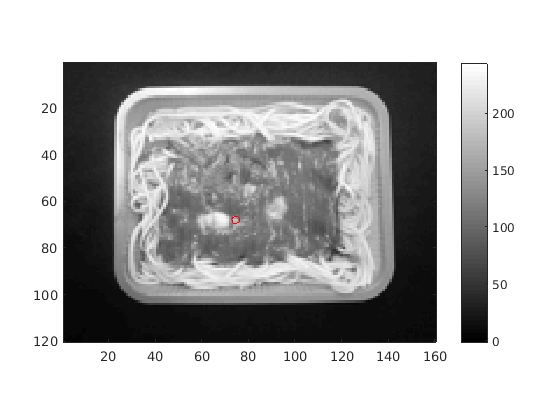
\includegraphics[width=60mm]{img/ex4/levelsets_bad.png}\label{fig:levelsets-bad}}
\subfigure[High $\nu$, low $\mu$]{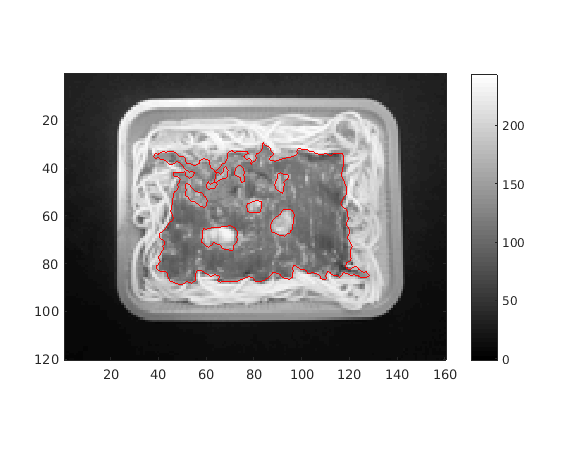
\includegraphics[width=60mm]{img/ex4/levelsets_more_or_less.png}\label{fig:levelsets-more-or-less}}

\subfigure[High $\mu$, low $\nu$. Best segmentation.]{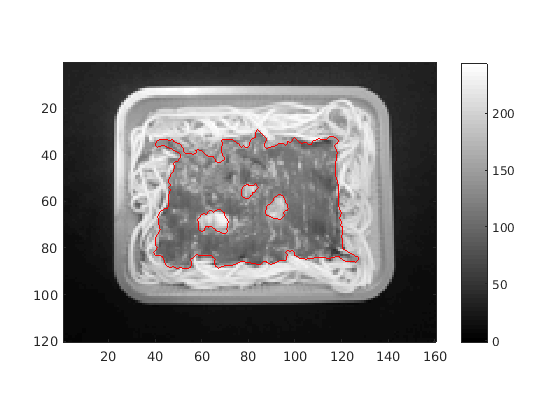
\includegraphics[width=60mm]{img/ex4/levelsets_good.png}\label{fig:levelsets-good}}

\caption{Segmentation of the dish with level sets}
\label{fig:levelsets-dish}
\end{figure}
